\begin{problem}[05]
求谐振子的自振频率.
\end{problem}
% --------------------------------------------------------------------
\begin{solution}
\begin{minipage}[c]{0.8\linewidth}
如右图所示, 谐振子的自振频率$f$仅与弹簧的弹性系数$k$及振子的质量$m$有关. 因此
\[
f = g(m,k)
\]
\end{minipage}
\begin{minipage}[c]{0.2\linewidth}
\begin{center}
\usetikzlibrary{%
    decorations.pathreplacing,%
    decorations.pathmorphing,arrows
}
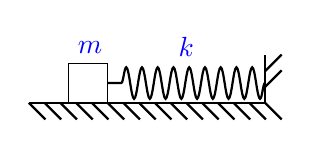
\begin{tikzpicture}[ media/.style={font={\footnotesize\sffamily}},
    wave/.style={
        decorate,decoration={snake,post length=1.4mm,amplitude=2mm,
        segment length=2mm},thick},
    interface/.style={
        postaction={draw,decorate,decoration={border,angle=-45,
                    amplitude=0.3cm,segment length=2mm}}}]
\draw[thick,interface](0,0)--(3,0)--(3,0.6);
\draw[wave](3,0.25)--(1,0.25) node[above=6pt,midway,blue]{$k$};
\draw  (1,0) rectangle (0.5,0.5) node[above right,blue]{$m$};

\end{tikzpicture}
\end{center}
\end{minipage}
上式中各物理量的量纲分别为: $[f] = T^{-1}$, $[m]=M$, $[k] = MT^{-2}$, 以$m$, $k$为基本量并作为单位, 有
\[
\frac{f}{\sqrt{k/m}} = g\bigg(\frac{m}{m},\frac{k}{k}\bigg) = g(1,1) = C
\]
其中$C$为常数, 因此谐振子的自振频率为: $f = C\sqrt{k/m}$. 理论上可得$C=2\pi$.
\end{solution}
